\documentclass{standalone}

\usepackage{tikz,xcolor}
\usetikzlibrary{shapes,shapes.geometric,shapes.symbols}
\usetikzlibrary{arrows, positioning, shapes.geometric, shapes.symbols}

\definecolor{mycolor}{RGB}{249,221,144}

\begin{document}
	
	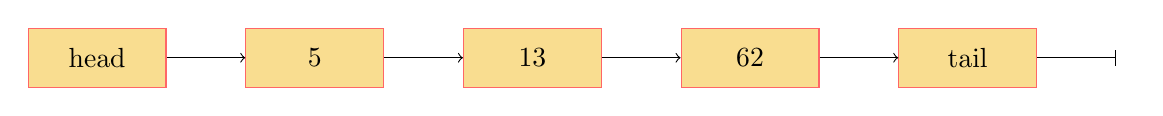
\begin{tikzpicture}[
		base/.style = {draw=red!60, fill=mycolor, minimum width=1.75cm, minimum height=0.75cm, align=center} , 
		node/.style = {rectangle, base}
		]
		\node (A) [node] {head};
		\node (B) [node,right=of A] {5};
		\node (C) [node,right=of B] {13};
		\node (D) [node,right=of C] {62};
		\node (E) [node,right=of D] {tail};
		\node (F) [right=of E] {};
		
		\draw[->] (A.east) -- (B.west);
		\draw[->] (B.east) -- (C.west);
		\draw[->] (C.east) -- (D.west);
		\draw[->] (D.east) -- (E.west);
		\draw[-|] (E.east) -- (F.west);
	\end{tikzpicture}
	
	
	
\end{document}